% Eigenvalue DOF-sweep spectra, colour variant (method by colour, DOF level by
% line style; index n vs eigenvalue lambda_n, several DOFs per method, against
% the analytic ground truth where available).
%
% Requires in the preamble:
%   \usepackage{graphicx}
%   \usepackage{subfig}
%
% The figures live next to this file, in results_paper/eigenvalues_dof_sweep/.
% If you \input this snippet from elsewhere, point graphicx at that folder, e.g.
%   \graphicspath{{results_paper/eigenvalues_dof_sweep/}}
% and drop the leading path from the \includegraphics arguments below.

\begin{figure}[htbp]
  \centering
  \subfloat[Rectangluar domain, \texttt{rectangle}.]{%
    
\includegraphics[width=0.8\textwidth]{rectangle_dof_sweep_colour}}
  \\
  \subfloat[Right isosceles triangle domain, \texttt{isosceles\_triangle}.]{%
    
\includegraphics[width=0.8\textwidth]{isosceles_triangle_dof_sweep_colour}}
  \caption{Eigenvalues of Laplace operator, zero Dirichlet boundary conditions. Comparison of analytical (exact) eigenvalues of the continuous eigenvalue problem and eigenvalues computed using various discretisations of Laplace operator; \texttt{FEM} -- finite element method, \texttt{FD} -- finite differences method, \texttt{Cheb} -- Chebyshev spectral collocation method, \texttt{DST} -- discrete sine transform method.}
  \label{fig:dof_sweep_colour}
\end{figure}

\begin{figure}[htbp]
  \centering
  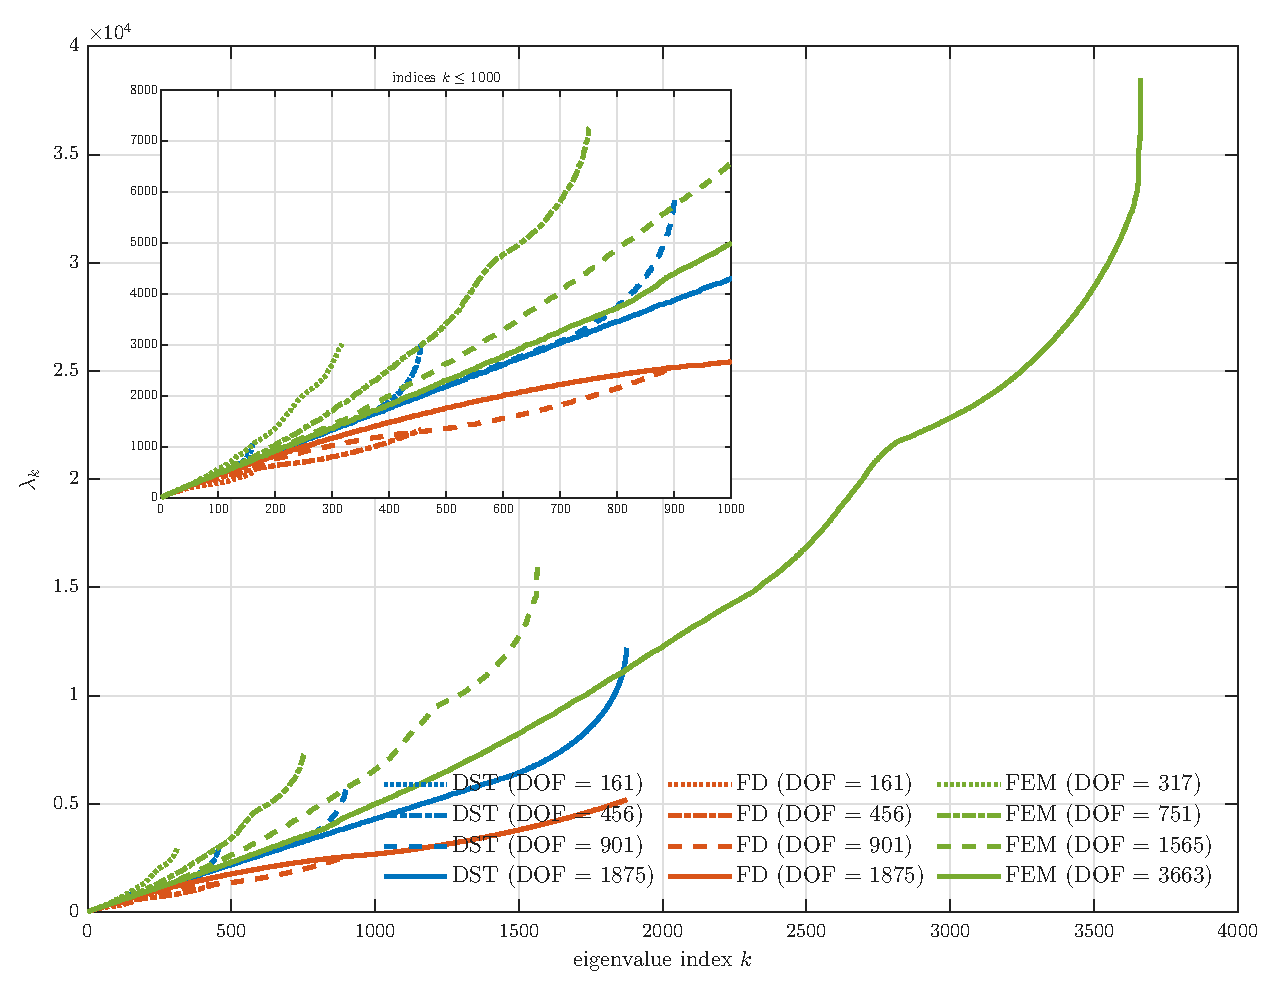
\includegraphics[width=0.8\textwidth]{L_shaped_dof_sweep_colour}
  \caption{Eigenvalues of Laplace operator, zero Dirichlet boundary conditions,  L-shaped domain \texttt{L\_shaped}. Eigenvalues computed using various discretisations of Laplace operator; \texttt{FEM} -- finite element method, \texttt{FD} -- finite differences method, \texttt{DST} -- discrete sine transform method.}
  \label{fig:dof_sweep_colour_L_shaped}
\end{figure}
